\section{Discussion}
\label{sec:4-discussion}
Maintenance scheduling efficiently solves a complex scheduling problem by the use of multiple actors. Through the use of actors the 
process handles uncertainty that is difficult to reason about, using models with different levels of aggregation where each actors understands
how to exploit his model. As uncertainties manifest themselves the actors/models handle the uncertainty through 
communication. To further understand the implications of the approach the discussion will be divided into three sections: 1. actors and 
integration; 2. continuous optimization allows asynchronous optimization; 3. future research.

\subsection{Actors \& Integration}
Often in operation research the failure to reliably solve industry problems are not due to the problems being computationally intractable 
but more a practical problem of connecting data streams so that the solution approach is connected to dynamic data source of the company
and then connecting the solution approach(s) to the relevant stakeholder (actors) through a relevant interface. The actor-based approach 
proposed in this paper makes integration easier by naturally encapsulation a model with a reliable interface. To better understand the 
novel properties of this consider the extension of figure 

\ref{fig:simple-maintenance-process}

as shown in figure \ref{fig:integrated:maintenance-process}.


\begin{figure}[H]
\centering
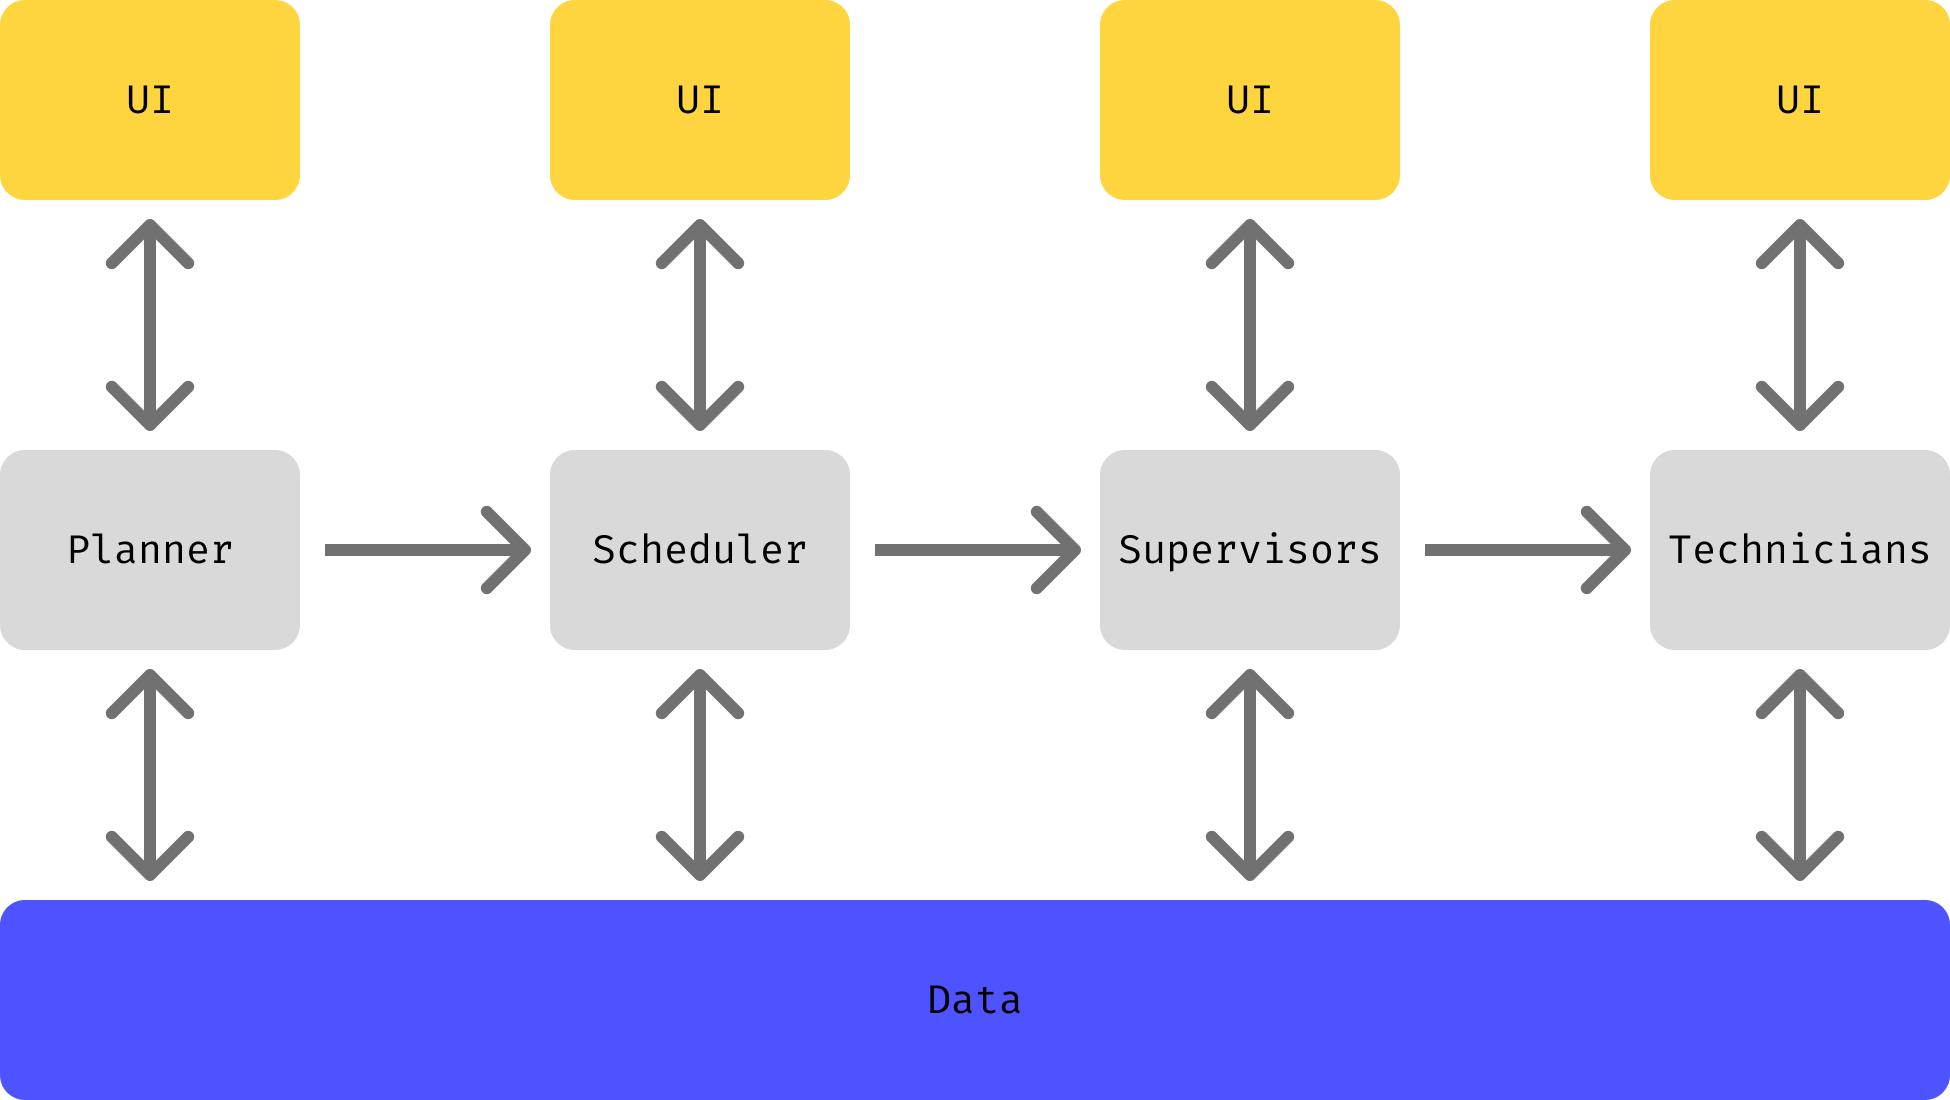
\includegraphics[width=1.0\textwidth]{figures/Scheduling Process Integrated.png}
\label{fig:integrated:maintenance-process}
\caption{Overview of the scheduling process when modelled as actors. When LNS is encapsulated 
is an actor it becomes possible to optimize parts of a large process individually instead of 
optimizing the scheduling problem globally from a single model inplementation.}
\end{figure}


\subsection{Continuous Optimization}
With actor-based metaheuristics it becomes simple to extend a metaheuristic to run
indefinitely with it being able to optimize based on the latest best 
available information. This may seem like a minor detail as you could argue that you should only ever optimize the schedule when there is 
an explicit need for it, but consider the case when you start adding more than two actor to a scheduling system, then there arises a need
to coordinate people in time as each will have to run their optimizer on after another.
